\section{Avance de proyecto especial}

Para el desarrollo del proyecto especial se contemplaron cuatro fases que consisten en:

\begin{itemize}
\item La primera fase corresponde a la consulta de diferentes algoritmos utilizados en el pre-procesamiento de datos en crudo de sistemas GPR, para ello se consultarán libros y artículos en bases de datos científicas
\item La segunda fase consiste en definir el tipo de algoritmo o el conjunto de algoritmos de pre-procesamiento a implementar para el GPR de laboratorio ubicado en la universidad de los Andes, este algoritmo será desarrollado en Matlab o Python.
\item La tercera fase corresponde a la implementación de diferentes pruebas con el GPR de laboratorio; serán ubicados diferentes objetos (metálicos y no metálicos) con el fin de obtener un banco de medidas en crudo para realizar el pre-procesamiento. Es importante que durante esta fase se documente de manera muy detallada las pruebas, porque se busca que las condiciones del laboratorio sean repetitivas para obtener los mismos resultados en cualquier momento
\item La cuarta fase corresponde a la implementación del algoritmo o el conjunto de algoritmos a las diferentes medidas realizadas con el GPR de laboratorio y validar mediante el análisis de resultados el rendimiento del algoritmo
\end{itemize}

\subsection{Calendario Propuesto}

\begin{figure}[H]
\centering
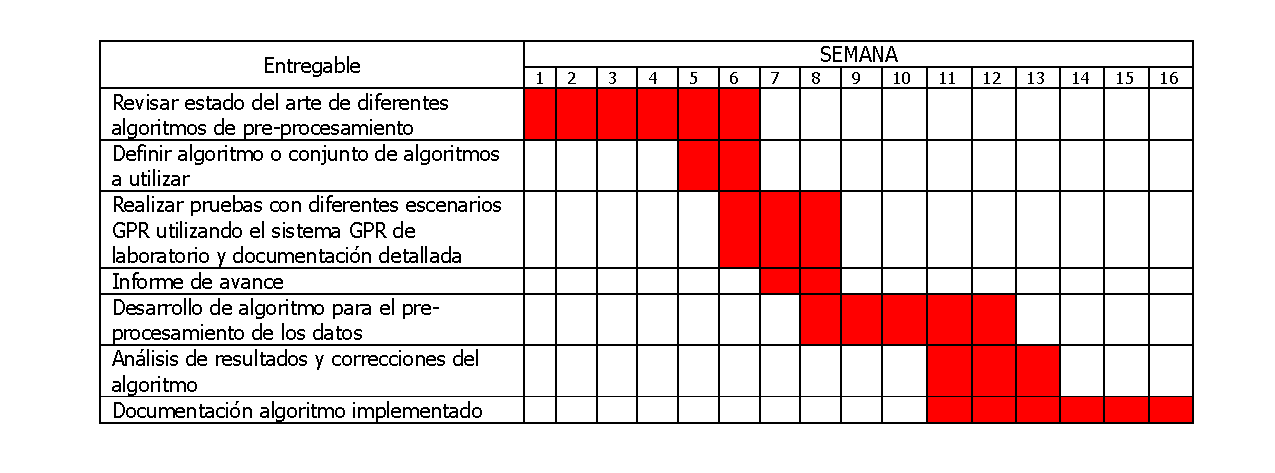
\includegraphics[height=6.5cm,keepaspectratio]{chapter2/images/Calendario_ProyectoEspecial.pdf}

\caption{Cronograma propuesto para Tesis I }
\label{fig:ch1_cronograma_propuesto_tesis}
\end{figure}


De acuerdo al calendario y fases propuestas, al día de la presentación del informe se ha realizado:

\begin{itemize}
\item Revisión del estado del arte de algoritmos de pre-procesamiento en bases de datos científica (IEEE) donde se revisó con el profesor Roberto Bustamante diferentes artículos que permitieran abordar el tema sin tener que recurrir a métodos extremadamente complejos para su desarrollo. 

\item Selección del algoritmo: En el cronograma se destinó la semana 5 y 6 para definir los algoritmos de pre-procesamiento; esta actividad se viene realizando desde el primer día de revisión de los artículos ya que era necesario revisar la implementación del algoritmo en Matlab a medida que se realizaba la lectura.

\item  Implementación de dos algoritmos de pre-procesamiento en las trazas obtenidas mediante simulación ya que se presento un inconveniente de adquisición de datos en medidas de laboratorio.  El VNA necesita estar calibrado,  en el laboratorio se están utilizando cables y antenas con conectores SMA pero el Kit de calibración solo es tipo N; se realizó la solicitud de cotización a la empresa Metricom del kit de calibración SMA, pero mientras se realiza esta compra se tomó la  decisión de utilizar datos simulados.

\item Simulaciones de diferentes modelos con objetos para aplicar los algoritmos de pre-procesamiento, estos resultados se encuentran más adelante. 

\end{itemize}




\subsection{Estado del arte}
Para la revisión del estado del arte inicialmente se realizó la lectura del capitulo 5 del libro \textit{Ground penetrating radar theory and applications} \cite{gpr_HarryM} donde contempla la etapa de procesamiento de datos GPR crudos (raw data) para eliminar el ruido que se presenta en cada una de las trazas proveniente de diferentes elementos presentes en un suelo, como lo es: el acople mutuo entre antenas (producido por la señal que llega directamente a la antena transmisora de la antena receptora), Las primeras reflexiones causadas por la interfaz aire-suelo, y las reflexiones causadas por elementos están enterrados bajo tierra y que pueden llegar a generar falsas alarmas. 

En este documento se presentan diferentes etapas de procesamiento tales como: interpolación del ``ruber-band''; filtro Dewow para eliminar componentes de frecuencia baja; Time-zero correction para corregir y ajustar un tiempo ``zero'' donde ocurre la primera reflexión en todas las trazas; filtrado; deconvolución; funciones de ganancia y migración.

En la universidad Louvain-la-Neuve (Belgica) , el instituto de tierra \cite{Detection_of_Reflection_Hyperbolas} desarrolló un método de detección de hipérbolas mediante filtros  donde la etapa de pre-procesamiento era importante para eliminar características constantes de que se presentaban en las trazas y luego llevar a cabo la detección de hiperboas mediante filtros Canny.

Raffaele Solimene et al. \cite{Ground_Clutter_Removal_in_GPR_Surveys} muestra como las reflexiones producidas por los suelos pueden impedir la detección de objetos enterrados debido a la magnitud de la señal y las frecuencias del sistema GPR, este tipo de ruido puede ser mitigado mediante la aplicación de algoritmos  basados en la entropía de los datos. En este documento se implementan dos etapas de pre-procesamiento, el ``Mean Substraction'' y el ``subspace projection'' para aplicar el método de entropía en la detección de ub objeto metalico de 26cm de largo y teniendo una sección trasversal de 4cm x 3cm enterrados a una distancia de 4cm; Utilizan un kit de radar (Ris-K2) que trabaja a una frecuencia de 2GHz, los resultados muestran que la aplicación de los algoritmos ``Mean Substraction'' y  ``subspace projection''  entregan resultados muy similares  y aplicando el metodo de entropia, supera el resultado de los dos algoritmos.

En la universidad nacional de defensa tecnológica Changsha, china \cite{Improving_RPCA-Based_Clutter_Suppression} implementaron un método novedoso para eliminar el ruido de los datos GPR en la detección de minas antipersonales basado en el algoritmo  ``Robust principal component analysis'' (RPCA). El algoritmo se encarga de separar las señales de ruido (Low-Rank) de la señales de los objetos (Sparse). Una vez implementado el algoritmo les permitió utilizar algoritmos de migración en las señales de los objetos (Sparse). Su trabajo concluye en que la combinación del algoritmo RPCA con el de migración es óptimo para separar las señales en ambientes con mucho clutter debido a su robustes.

Priyadarshini et al. \cite{Buried-Discrimination-gpr-Radar-Radargram} implementa un método para discriminar las señales clutter de los objetos en las señales GPR aplicando dos etapas de pre procesamiento y un análisis espectral para determinar si el objeto si es una mina.

En la etapa de pre-procesamiento utiliza el algoritmo ``Ensamble Averaging''  que es el mismo ``Mean Substraction'' de los otros articulos encontrados. Una vez aplica dicho algoritmo, implementa un algoritmo en cascada llamado ``Entropy Optimized Contrast Stretching'' mediante los algoritmos  ``Contrast Stretching'' (CS) y ``Entropy Optimized'' para hacer un mejor uso del rango dinámico de la imagen y de esta manera se pueda apreciar mejor las hipérbolas en las trazas B.

Como resultado de dicho trabajo es la eliminación del clutter y mejorando la imagen de la traza B para poder discriminar objetos de diferentes tamaños, con dichos resultados, le permitió aplicar algoritmos métodos de detección mediante técnicas de análisis espectral.

Por último Anonios Giannopolus et al. crean un modelo basado en inteligencia artificial mediante redes neuronales  para entrenar un algoritmo que sea capaz de reconocer las señales provenientes de un ojeto y discriminar las señales de ruido en tiempo real \cite{gprMax,Evaluation_of_Signal-to-Clutter_Ratio}

\subsection{Algoritmos Implementados}

De acuerdo con la revisión del estado del arte y de acuerdo a los resultados obtenidos se ha decidido utilizar algunos de los algoritmos mencionados, por ejemplo, el algoritmo utilizado en \cite{Improving_RPCA-Based_Clutter_Suppression} demuestra una gran utilidad para separar el ruido de la señal de la mina (target) u otro objeto a sin conocer las condiciones del suelo, lo que es de gran utilidad al momento de usar un sistema GPR.

Por otro lado se utilizó también el algoritmo ``Mean Substraction'' ya que a pesar que es uno de los algoritmos mas sencillos, es utilizado lo la mayoría de los artículos. A continuación se mostrará el desarrollo de cada uno de los algoritmos en las señales de los modelos simulados.
\subsubsection{Robust PCA}
Robust Principal Component Analysis es un algoritmo  desarrollado en conjunto por la universidad de Illinois y  Standford \cite{Candes:RPCA} que fue utilizado inicialmente en aplicaciones de visión por computador. En la actualidad uno de los problemas al analizar datos es poder extraer información intrínseca de un conjunto de datos. 

\begin{figure}[H]
\centering
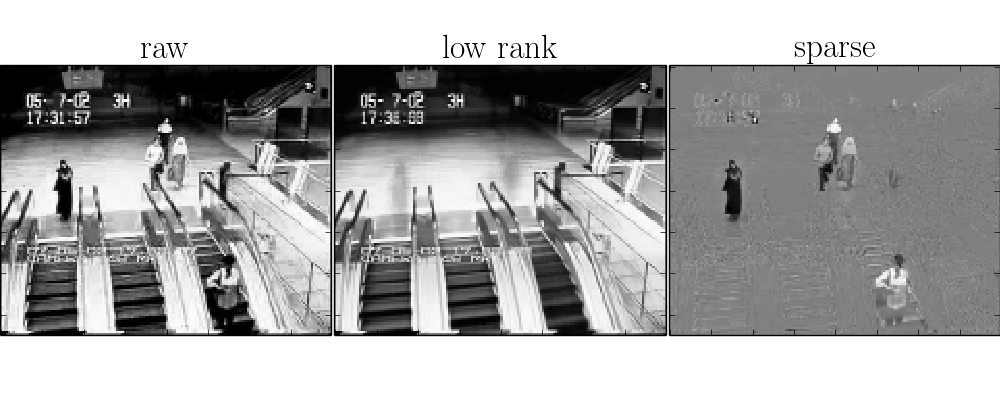
\includegraphics[height=6.5cm,keepaspectratio]{chapter2/images/example_RPCA.png}

\caption{Ejemplo RPCA en aplicaciones de vídeo }
\label{fig:example_rpca}
\end{figure}

El uso de este algoritmo es de gran importancia en las aplicaciones de GPR para eliminar clutter sin conocer las propiedades del suelo que esta bajo medición.

Matemáticamente, RPCA puede ser observada como una matriz D de la siguiente forma:

\begin{equation}
    D=L+S+N
    \label{eq:rpca_general}
\end{equation}

Donde \textbf{L} indica la matriz Low-Rank o Background que representa todas las señales de fondo, para GPR estas señales pueden ser las múltiples reflexiones en la interfaz aire-suelo y el acople entre antenas; \textbf{S} la matriz Sparse son los objetos en primer plano  que correspoderían a todas las señales propias de las minas (target)   y \textbf{N} un termino de ruido. En \cite{rpca_review}  no se tiene en cuenta ya que se puede ver \textbf{L} y \textbf{N} como un solo valor.

Las secuencias que se presentan en el fondo puede ser modeladas como un sub espacio que cambia gradualmente con respecto al tiempo (Matriz \textbf{L}), mientras que los objetos en movimiento constituyen eventos atípicos que pueden ser correlacionados.


La matriz D se puede descomponer como el siguiete problema de optimización:
\begin{equation}
\min _{ L,S }{ { \left\| L \right\|  }_{ * } } +\lambda {\left\| S \right\| }_{1}\quad \quad  con \quad   restricción\quad  D-L-S=0
\label{eq:minimizar}
\end{equation}


Donde  la norma ${ \left\|  \bullet \right\|  }$ (nuclear norm) corresponde a la la suma de los valores singulares de la matriz L y ${ \left\|  \bullet  \right\|  }_{1}$ es la norma $l^1$ de una matriz vista como vector, este valor es calculado como la suma de los valores absolutos de la matriz D.  $\lambda $  corresponde a un multiplicador lagrangiano 

\subsubsubsection{\textbf{Implementación RPCA en trazas gprMax}}

Se desarrolló en Matlab un algoritmo que permitiera seleccionar una cantidad N de trazas B para aplicarle a cada componente de campo (Ex,Ey,Ez,Hx,Hy,Hz) el algoritmo RPCA, el código implementado es el siguiente:

\begin{lstlisting}[ basicstyle=\tiny]
% get_RPCA_Bscans.m
% Los Andes University
% Creaded By: Luis Eduardo Quibano Alarcon
% E-mail: le.quibano@uniandes.edu.co
% Description: This Script  opens a specific amoun of  Bscans in order to
%              apply them the RPCA algotrithm in all field  components of
%              each A-scan, The result of this algorithm gives L and S
%              matrixes; create a new set of B_scans of the resulting
%              matrixes L and S
% RPCA algoithm : https://statweb.stanford.edu/~candes/papers/RobustPCA.pdf
% Original Github Repository: https://github.com/dlaptev/RobustPCA

clear all
close all
clc

[filename, pathname] = uigetfile('*.out', 'Select gprMax B-scans output files','MultiSelect','on');
fullfilename = strcat(pathname, filename);

filename = cellstr(filename);
pathname = cellstr(pathname);
fullfilename = cellstr(fullfilename);

%Extraigo todos los campos de los A-scan seleccionados y luego los guardo
%en la matriz del objeto fields{i}
if length(fullfilename) ~=0
    for i=1:length(fullfilename)
        if filename{i} ~= 0
            iterations = double(h5readatt(fullfilename{i}, '/', 'Iterations'));
            dt = h5readatt(fullfilename{i}, '/', 'dt');
            
            ExFieldPath = strcat('/rxs/rx1/', 'Ex');
            EyFieldPath = strcat('/rxs/rx1/', 'Ey');
            EzFieldPath = strcat('/rxs/rx1/', 'Ez');
            HxFieldPath = strcat('/rxs/rx1/', 'Hx');
            HyFieldPath = strcat('/rxs/rx1/', 'Hy');
            HzFieldPath = strcat('/rxs/rx1/', 'Hz');
            
            
            ExAllScans = h5read(fullfilename{i}, ExFieldPath);
            EyAllScans = h5read(fullfilename{i}, EyFieldPath);
            EzAllScans = h5read(fullfilename{i}, EzFieldPath);
            HxAllScans = h5read(fullfilename{i}, HxFieldPath);
            HyAllScans = h5read(fullfilename{i}, HyFieldPath);
            HzAllScans = h5read(fullfilename{i}, HzFieldPath);
            
            %% APPLY RPCA
            [L_ExAllScans,S_ExAllScans] = getRPCAinComponent('ex',ExAllScans);
            [L_EyAllScans,S_EyAllScans] = getRPCAinComponent('ey',EyAllScans);
            [L_EzAllScans,S_EzAllScans] = getRPCAinComponent('ez',EzAllScans);
            [L_HxAllScans,S_HxAllScans] = getRPCAinComponent('hx',HxAllScans);
            [L_HyAllScans,S_HyAllScans] = getRPCAinComponent('hy',HyAllScans);
            [L_HzAllScans,S_HzAllScans] = getRPCAinComponent('hz',HzAllScans);
            
            %% Create New A-scan set with LowRank And Spare Results
            %Como ya tengo los resultados del algoritmo (L y S) creo los mismos
            %creo los mismos archivos
            generate_LowRank
            generate_Sparse
        end
    end
    
end

%% Funcion del algoritmo RPCA
function [L,S] = getRPCAinComponent(component,data)
%Los datos deben trabajarse de forma normalizada para ello se realiza el
%proceso de encontrar el mayor valor y el menor valor
minVal = min(min(data));
maxVal = max(max(data));
X_norm = (data - minVal) / ( maxVal - minVal );
%Aplicar RPCA
lambda = 1/sqrt(max(size(X_norm)));
tic
[L_norm,S_norm] = RobustPCA(component,X_norm, (lambda/3)*1.5 , ((10*lambda)/3)*1.5, 1e-5,1000);
toc %Me indica el tiempo que tardo en realizar RPCA a los datos de entrada con mil iteraciones
%El resultado del alogoritmo me entrega los de la matriz L y S de forma
%normalizada, para ello, encuentro el valor real.
%los datos de L y S se devuelven en la funcion y son los que se van a
%graficar
L=L_norm.*( maxVal - minVal ) + minVal;
S=S_norm.*( maxVal - minVal ) + minVal;
end
\end{lstlisting}

Como se puede observar se utiliza la función \textit{getRPCAinComponen()} donde su parámetro de entrada son los valores de campo. Más adelante se puede observar que antes de aplicar el algoritmo como tal, los datos necesitan ser normalizados, esta es una condición especial del algoritmo,  así mismo es necesario indicar el valor de $\lambda $, si este valor no es puesto como parámetro, este tomara el valor por defecto de $ 1 / sqrt(max(M,N)$. Una vez los datos se encuentran normalizados los datos entran a la función \textit{RobustPCA()}, esta función entrega como resultados los valores de las matrices $L$ y $S$ normalizadas, estas dos matrices se desnormalizan para obtener los valores originales de campo.


\begin{lstlisting}[ basicstyle=\tiny]
function [L, S] = RobustPCA(component,X, lambda, mu, tol, max_iter)
    % - component is the string of the name of the component which is
    % applied RPCA
    % - X is a data matrix (of the size N x M) to be decomposed
    %   X can also contain NaN's for unobserved values
    % - lambda - regularization parameter, default = 1/sqrt(max(N,M))
    % - mu - the augmented lagrangian parameter, default = 10*lambda
    % - tol - reconstruction error tolerance, default = 1e-6
    % - max_iter - maximum number of iterations, default = 1000

    [M, N] = size(X);
    unobserved = isnan(X);
    X(unobserved) = 0;
    normX = norm(X, 'fro');

    % default arguments
    if nargin < 2
        lambda = 1 / sqrt(max(M,N));
    end
    if nargin < 3
        mu = 10*lambda;
    end
    if nargin < 4
        tol = 1e-6;
    end
    if nargin < 5
        max_iter = 1000;
    end
    
    % initial solution
    L = zeros(M, N);
    S = zeros(M, N);
    Y = zeros(M, N);
    
    for iter = (1:max_iter)
        % ADMM step: update L and S
        L = Do(1/mu, X - S + (1/mu)*Y);
        S = So(lambda/mu, X - L + (1/mu)*Y);
        % and augmented lagrangian multiplier
        Z = X - L - S;
        Z(unobserved) = 0; % skip missing values
        Y = Y + mu*Z;
        
        err = norm(Z, 'fro') / normX;
        if (iter == 1) || (mod(iter, 10) == 0) || (err < tol)
            fprintf(1, 'component: %s   iter: %04d\terr: %f\trank(L): %d\tcard(S): %d\n', ...
                    component,iter, err, rank(L), nnz(S(~unobserved)));
        end
        if (err < tol) break; end
    end
end
function r = So(tau, X)
    % shrinkage operator
    r = sign(X) .* max(abs(X) - tau, 0);
end
function r = Do(tau, X)
    % shrinkage operator for singular values
    [U, S, V] = svd(X, 'econ');
    r = U*So(tau, S)*V';
end
\end{lstlisting}

En la siguientes lineas de códigos se encargan de tomar los datos de la matriz L y crear una nueva traza B y guardarlo en una nueva carpeta de mediciones.

\begin{lstlisting}[ basicstyle=\tiny]

% clear all, clc
% close all
% load('matlab.mat')
fullfilenameLowRank = fullfilename{i};
filenameLowRank=filename{i};
%%CREATE A COPY OF B-SCAN WITH NAME LOW RANK
%%SI LA ITERACION ES LA 1, borrar todas las carpetas y empezar a crear los
%%archivos
if i==1
    if exist(strcat(pathname{1},'/lowrank_bscan')) == 7
        rmdir(strcat(pathname{1},'/lowrank_bscan'), 's')
    end
    mkdir(strcat(pathname{1},'/lowrank_bscan'))
end
pathToSave=strcat(pathname{1},'/lowrank_bscan')


nameSplit = split(filenameLowRank,'.');
nameSplit= nameSplit(1);
nameSplit= strcat(pathToSave,'/',nameSplit{1});
nameSplit=strcat(nameSplit(1:end),'_LowRank','.out');
fullfilenameLowRank=nameSplit ;
copyfile(fullfilename{i}, nameSplit);



%%Modify All LowRank Files

iterations = double(h5readatt(fullfilenameLowRank, '/', 'Iterations'));
dt = h5readatt(fullfilenameLowRank, '/', 'dt');

ExFieldPath = strcat('/rxs/rx1/', 'Ex');
EyFieldPath = strcat('/rxs/rx1/', 'Ey');
EzFieldPath = strcat('/rxs/rx1/', 'Ez');
HxFieldPath = strcat('/rxs/rx1/', 'Hx');
HyFieldPath = strcat('/rxs/rx1/', 'Hy');
HzFieldPath = strcat('/rxs/rx1/', 'Hz');

h5write(fullfilenameLowRank, ExFieldPath,L_ExAllScans);
h5write(fullfilenameLowRank, EyFieldPath,L_EyAllScans);
h5write(fullfilenameLowRank, EzFieldPath,L_EzAllScans);
h5write(fullfilenameLowRank, HxFieldPath,L_HxAllScans);
h5write(fullfilenameLowRank, HyFieldPath,L_HyAllScans);
h5write(fullfilenameLowRank, HzFieldPath,L_HzAllScans);
\end{lstlisting}

De la misma manera ocurre para guardar las trazas B de la matriz S.

\begin{lstlisting}[ basicstyle=\tiny]
%
% clear all, clc
% close all
% load('matlab.mat')
fullfilenameSparse = fullfilename{i};
filenameSparse=filename{i};
%%CREATE A COPY OF B-SCAN WITH NAME LOW RANK
%%SI LA ITERACION ES LA 1, borrar todas las carpetas y empezar a crear los
%%archivos
if i==1
    if exist(strcat(pathname{1},'/sparse_bscan')) == 7
        rmdir(strcat(pathname{1},'/sparse_bscan'), 's')
    end
    mkdir(strcat(pathname{1},'/sparse_bscan'))
end
pathToSave=strcat(pathname{1},'/sparse_bscan')
nameSplit = split(filenameSparse,'.');
nameSplit= nameSplit(1);
nameSplit= strcat(pathToSave,'/',nameSplit{1});
nameSplit=strcat(nameSplit(1:end),'_Sparse','.out');
fullfilenameSparse=nameSplit ;
copyfile(fullfilename{i}, nameSplit);
%%Modify All LowRank Files
iterations = double(h5readatt(fullfilenameSparse, '/', 'Iterations'));
dt = h5readatt(fullfilenameSparse, '/', 'dt');
ExFieldPath = strcat('/rxs/rx1/', 'Ex');
EyFieldPath = strcat('/rxs/rx1/', 'Ey');
EzFieldPath = strcat('/rxs/rx1/', 'Ez');
HxFieldPath = strcat('/rxs/rx1/', 'Hx');
HyFieldPath = strcat('/rxs/rx1/', 'Hy');
HzFieldPath = strcat('/rxs/rx1/', 'Hz');
h5write(fullfilenameSparse, ExFieldPath,S_ExAllScans);
h5write(fullfilenameSparse, EyFieldPath,S_EyAllScans);
h5write(fullfilenameSparse, EzFieldPath,S_EzAllScans);
h5write(fullfilenameSparse, HxFieldPath,S_HxAllScans);
h5write(fullfilenameSparse, HyFieldPath,S_HyAllScans);
h5write(fullfilenameSparse, HzFieldPath,S_HzAllScans);

\end{lstlisting}

En la \figurename{ \ref{fig:results_rpca_folders}} se muestra como se organizan los resultados una vez aplicado el algoritmo RPCA sobre las trazas B, el programa en Matlab se encarga de crear una carpeta llamada \textbf{lowrank\_bcscan} y otra llamada \textbf{sparse\_bscan}
\begin{figure}[H]
\centering
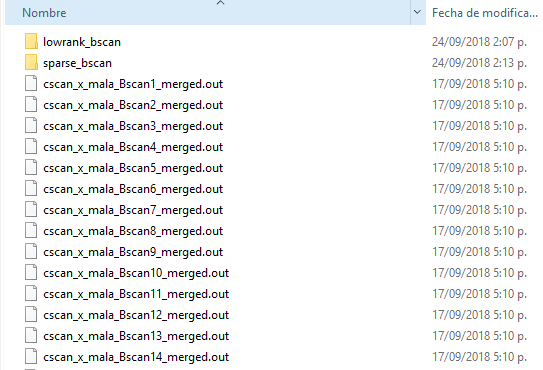
\includegraphics[height=5.5cm,keepaspectratio]{chapter2/images/resultado_rpca_trazasB.png}
\caption{Carpeta de resultados después de aplicar RPCA a las trazas B originales }
\label{fig:results_rpca_folders}
\end{figure}


A continuación se muestra el resultado de aplicar RPCA sobre un modelo de 0.5mx0.5mx0.4m de dominio, con resolución de 0.002m, se utiliza una antena MALA y de desplaza 0.005m en cada iteración.

Se Aplica RPCA a cada componente, pero vamos a observar la señal sobre Ez. En la \figurename{ \ref{fig:bscanRPCA_SIM1}} se observa el resultado del modelo, la traza B original,  y los resultados de extraer el ruido de fondo y la señal de las barras metálicas.



\begin{figure}[H]  
\centering
\subfigure[ Modelo Original ]{
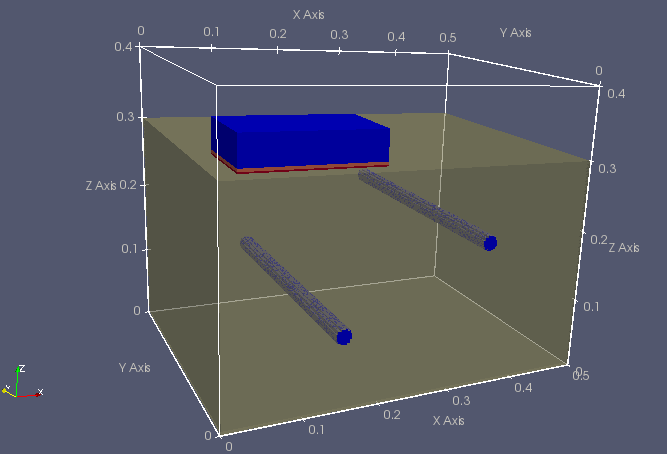
\includegraphics[width=0.35\textwidth, keepaspectratio,valign=c]{chapter2/images/mala_2_barras.png}
\label{fig:subfig_mala2_barras_mod}
}
\subfigure[ Bscan datos crudos ]{
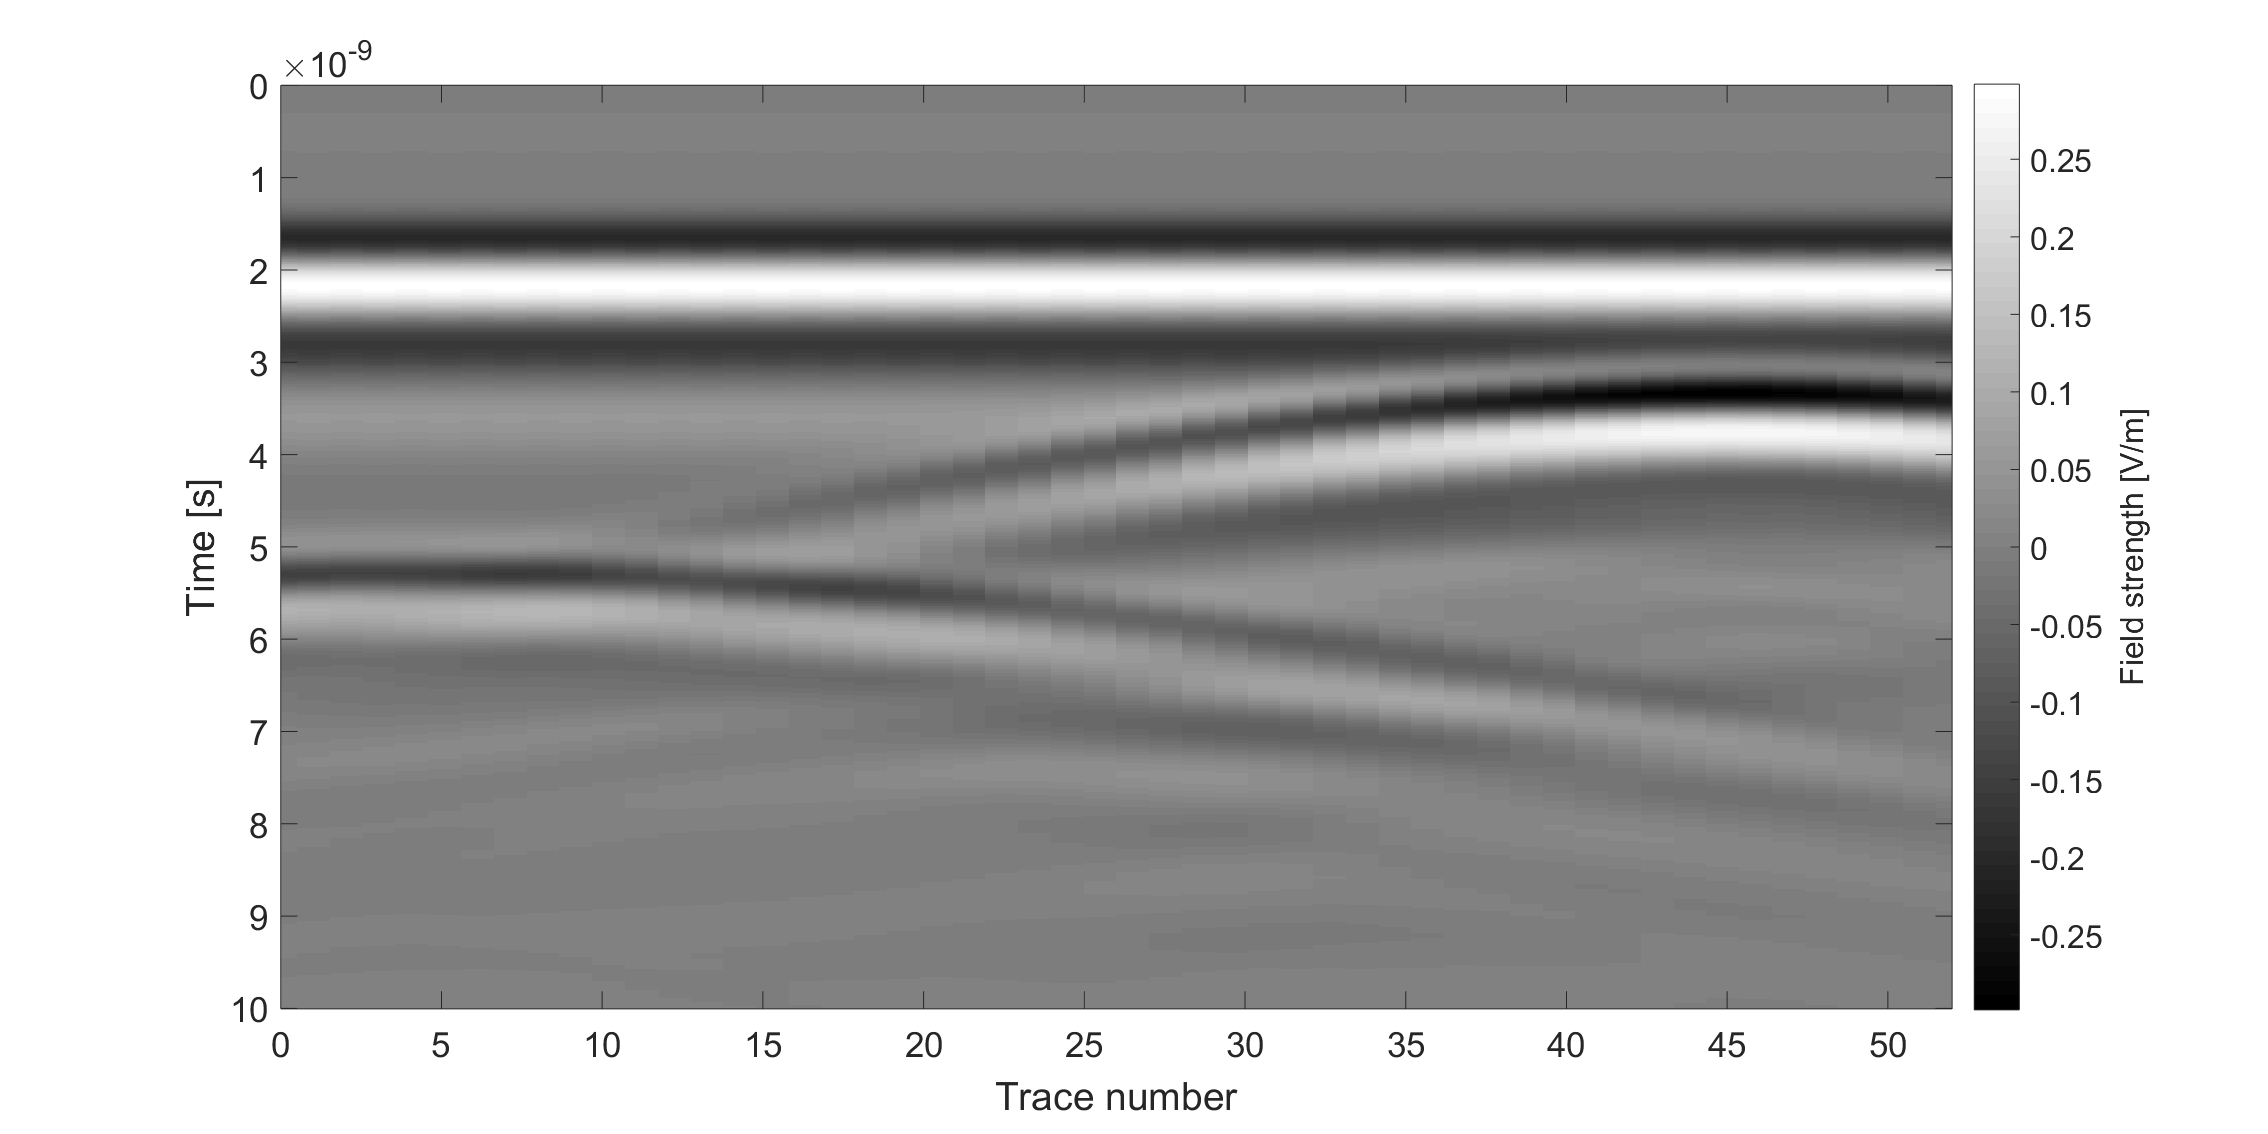
\includegraphics[width=0.55\textwidth, keepaspectratio,valign=c]{chapter2/images/mala_2_barras_bscan.png}
\label{fig:subfig1xampleCscan1GSSI}
} \\
\subfigure[ Bscan Low Rank ]{
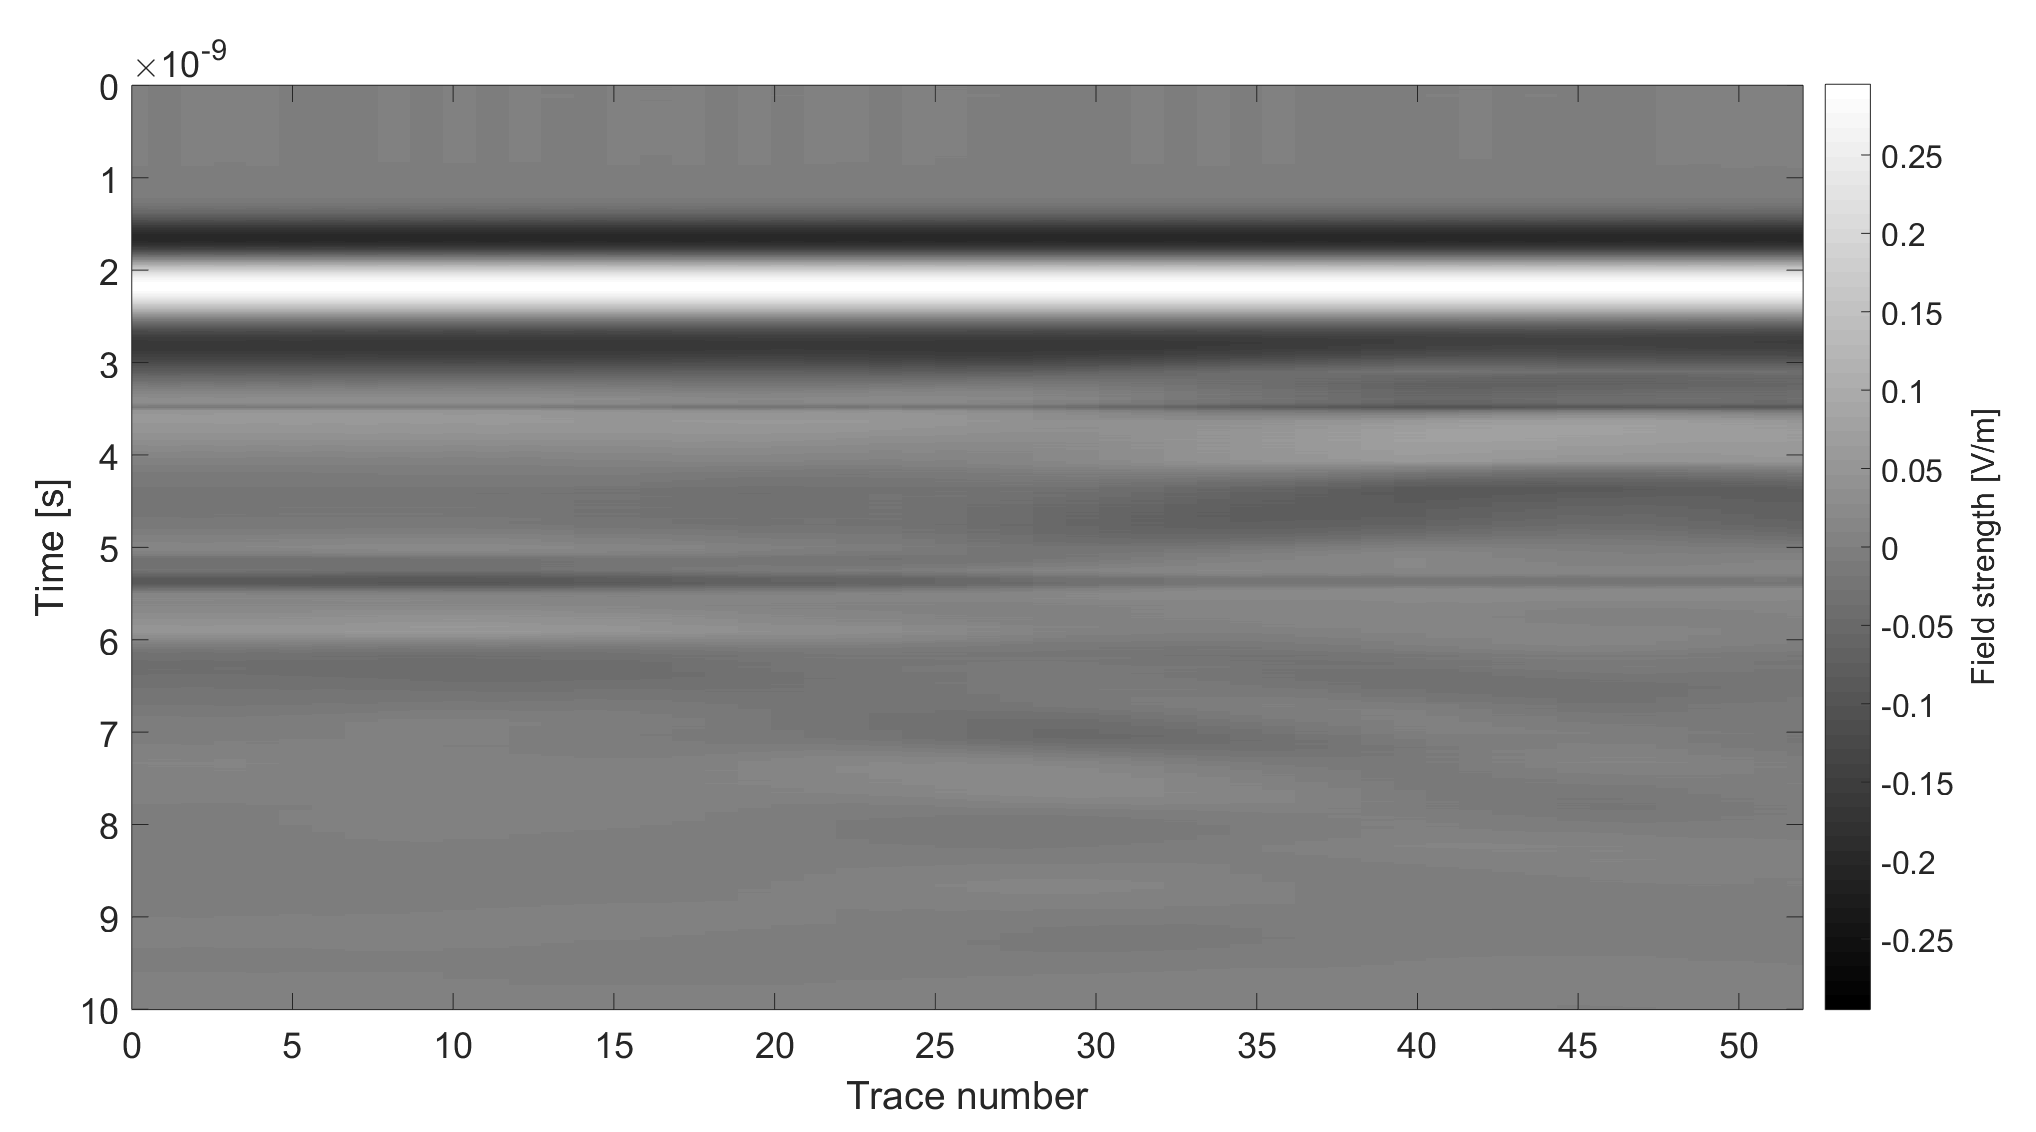
\includegraphics[width=0.47\textwidth, keepaspectratio,valign=c]{chapter2/images/mala_2_barras_bscan_low.png}
\label{fig:subfig2exampleCscan1GSSI}
}
\subfigure[Bscan Sparse ]{
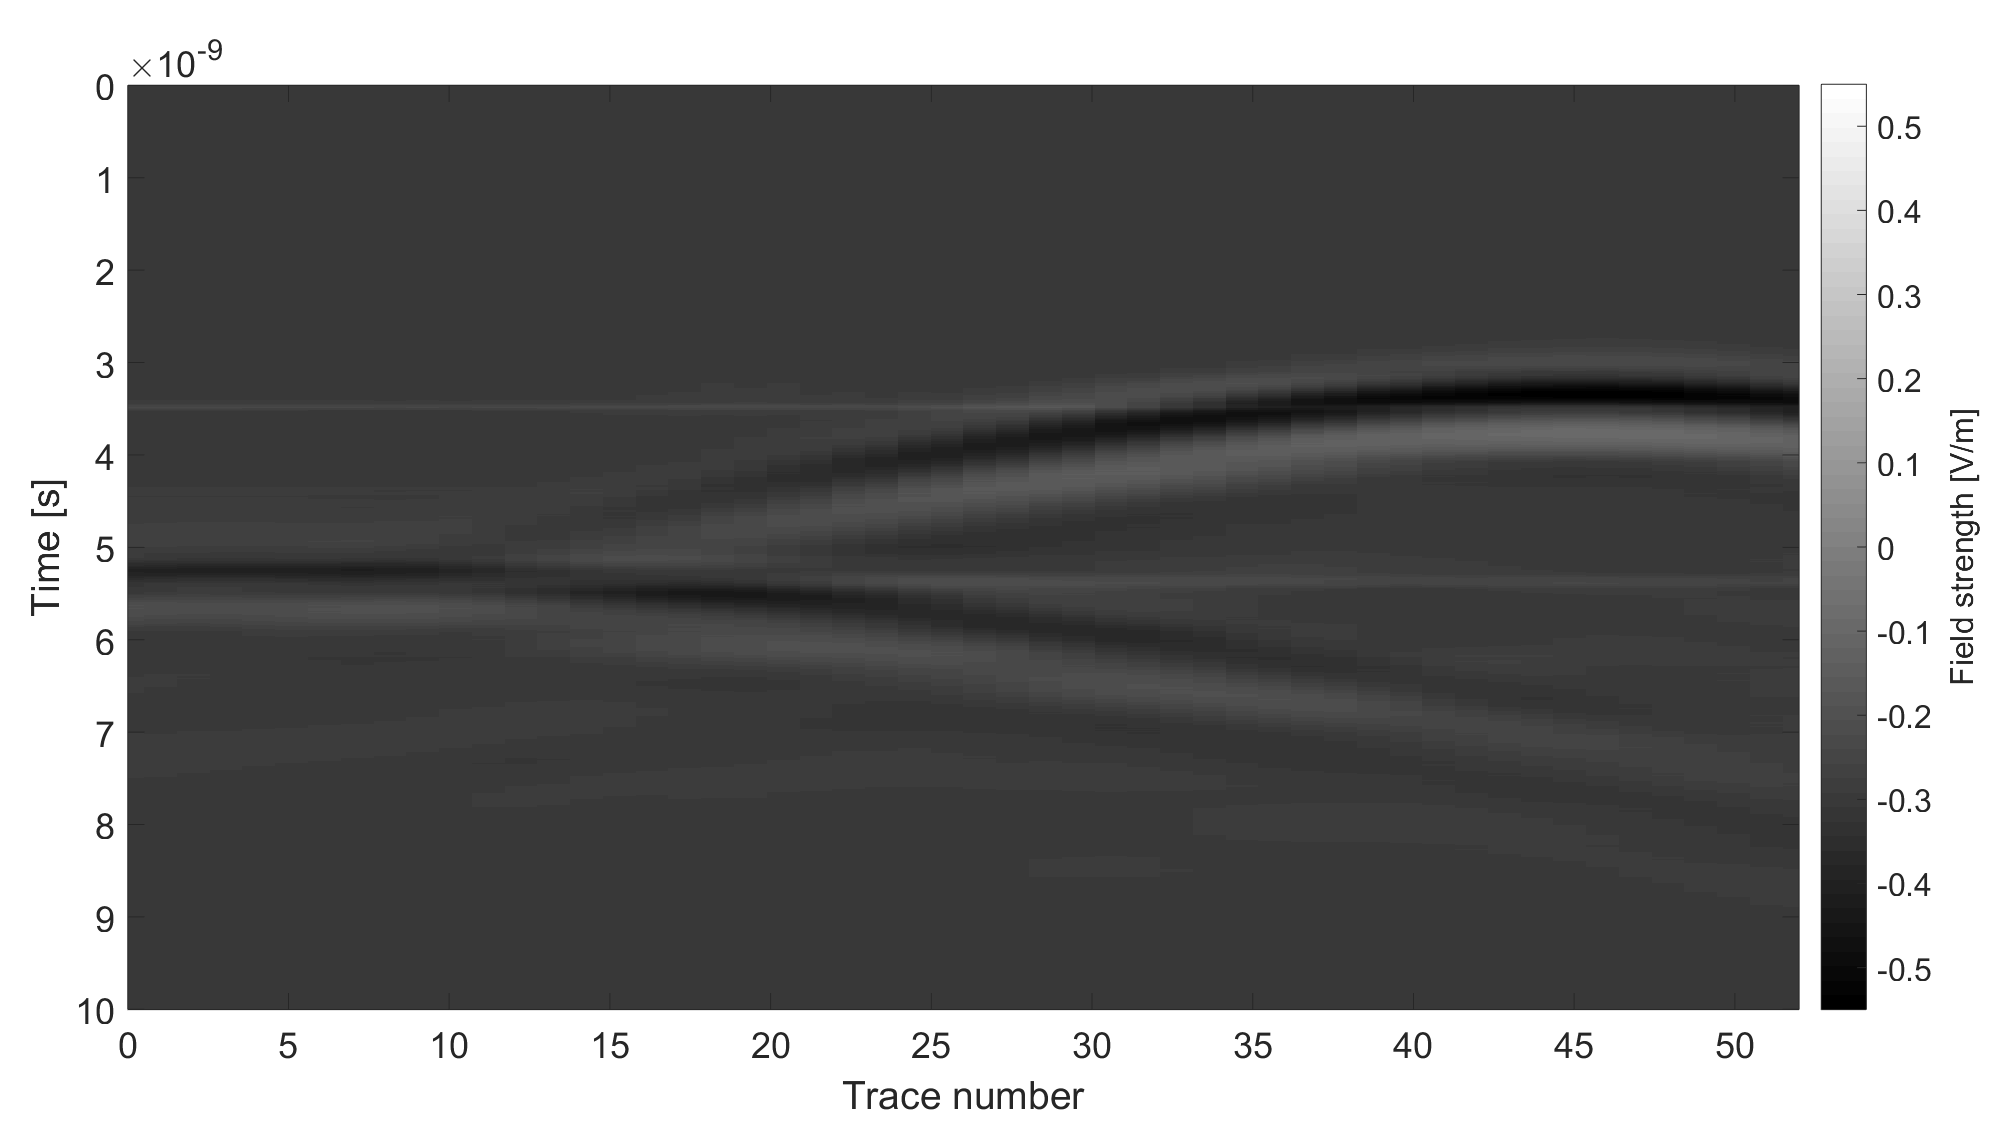
\includegraphics[width=0.47\textwidth, keepaspectratio,valign=c]{chapter2/images/mala_2_barras_bscan_sparse.png}
}

\caption{RPCA sobre trazas B en campo Ez}
\label{fig:bscanRPCA_SIM1}


\end{figure}

Para saber qué tan perfecta debe ser la señal extraída, se procede a realizar la simulación del mismo escenario pero sin barras metálicas. Al resultado de la traza B con todos los elementos le es restado la traza B con solo el suelo para tener como resultado la señal de las barras metálicas.

Para encontrar qué tan parecida es la señal de la traza B después de aplicar RPCA con la señal ``ideal''   matemáticamente podemos utilizar el índice de correlación.  Se realiza un programa en Matlab que permita cargar dos trazas B y a ellas le aplica el índice de correlación a todos los campos. Como resultado del ejemplo en medición se tiene:


\begin{table}[H]
\begin{center}
\caption{Similitud entre resultados aplicando RPCA} \label{tab:corrcoef1}
\begin{tabular}{l|c}
 & \multicolumn{1}{l}{\textbf{Índice de Correlación}} \\ \hline
\textbf{(Ex ideal,Ex Sparse)} & NaN \\
\textbf{(Ey ideal,Ey Sparse)} & 0.8482 \\
\textbf{(Ez ideal,Ez Sparse)} & 0.8482 \\
\textbf{(Hx ideal,Hx Sparse)} & 0.7593 \\
\textbf{(Hy ideal,Hy Sparse)} & 0.9670 \\
\textbf{(Hz ideal,Hz Sparse)} & 0.9703
\end{tabular}
\end{center}
\end{table} 

\begin{figure}[H]  
\centering
\subfigure[ Bscan Ideal ]{
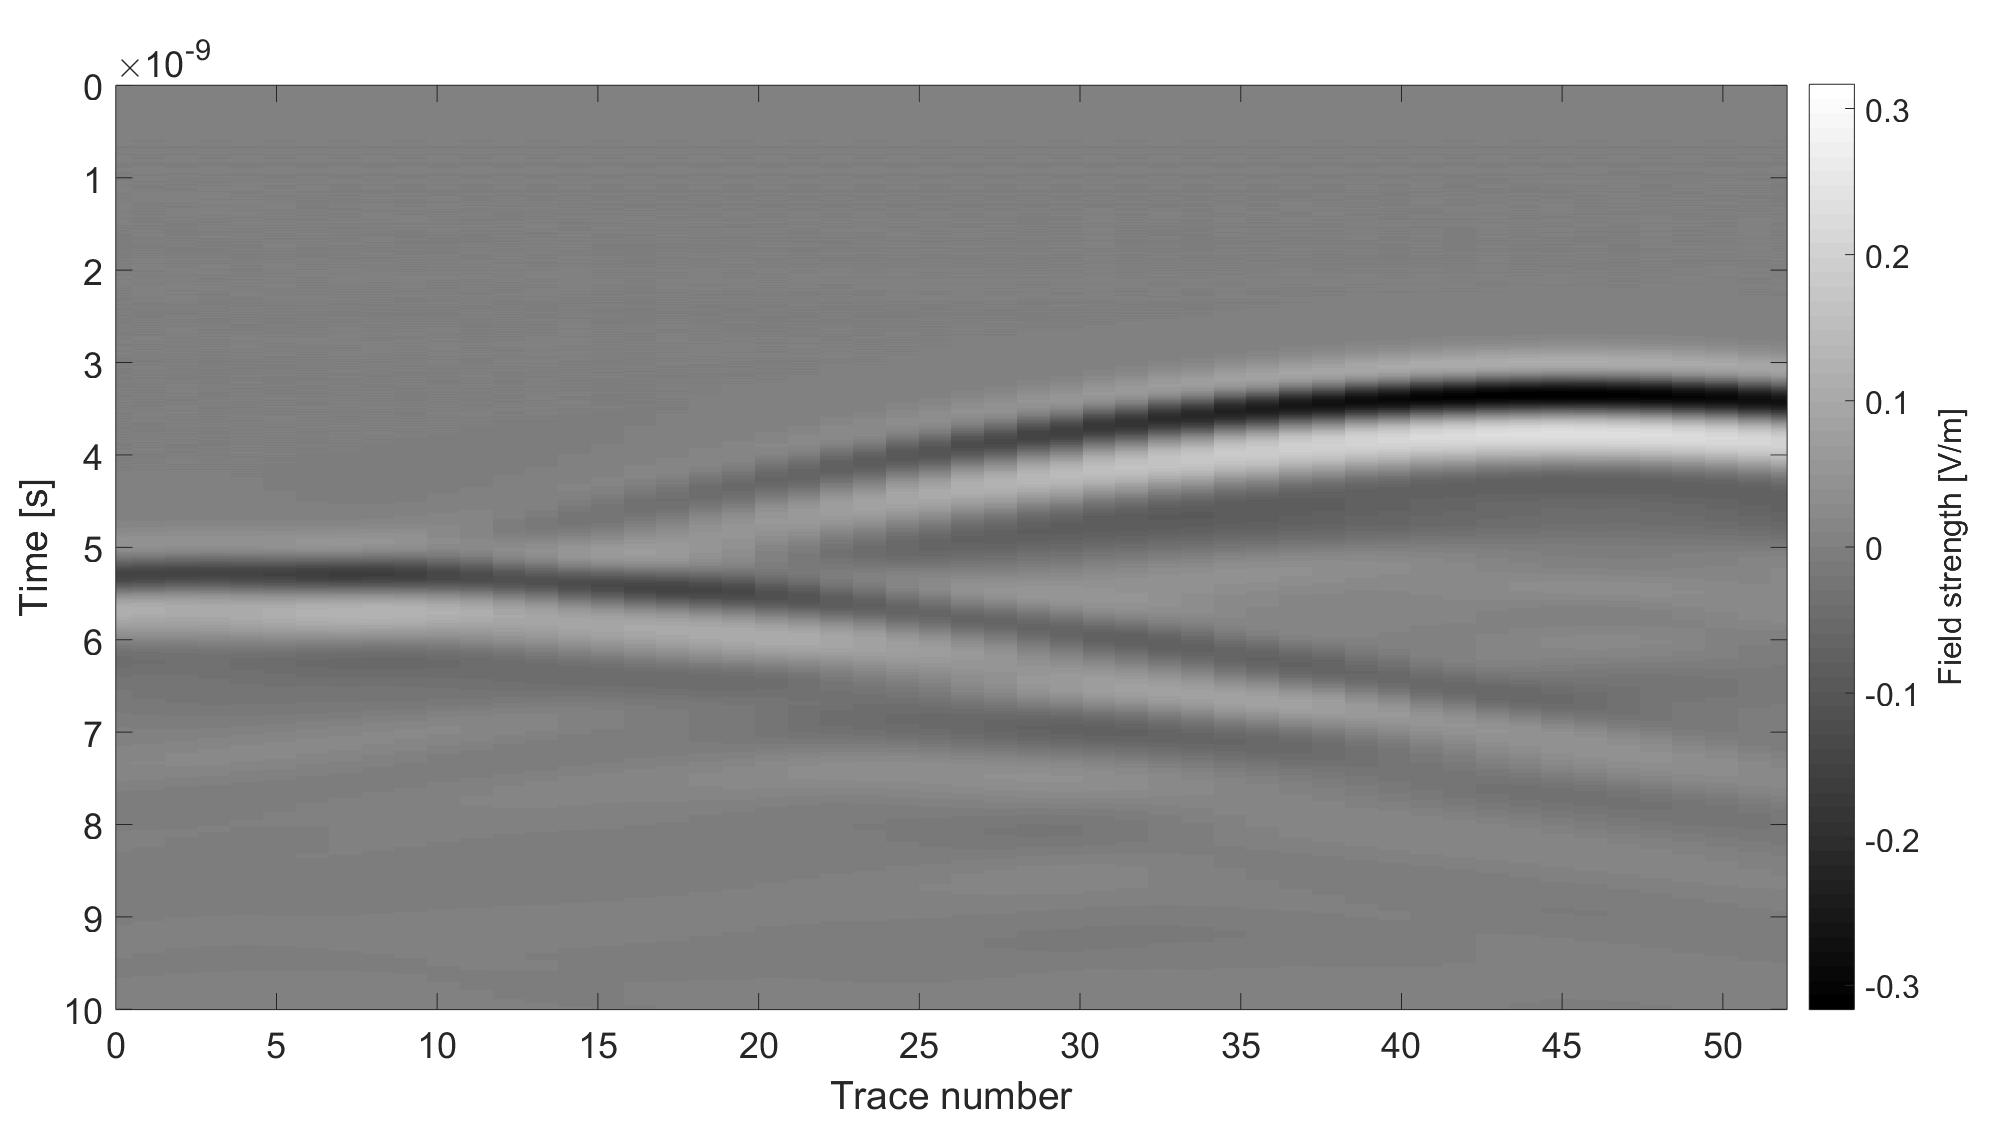
\includegraphics[width=0.47\textwidth, keepaspectratio,valign=c]{chapter2/images/mala_2_barras_bscan_sparse_ideal.png}
\label{fig:subfig2exampleCscan1GSSI}
}
\subfigure[Bscan Sparse ]{
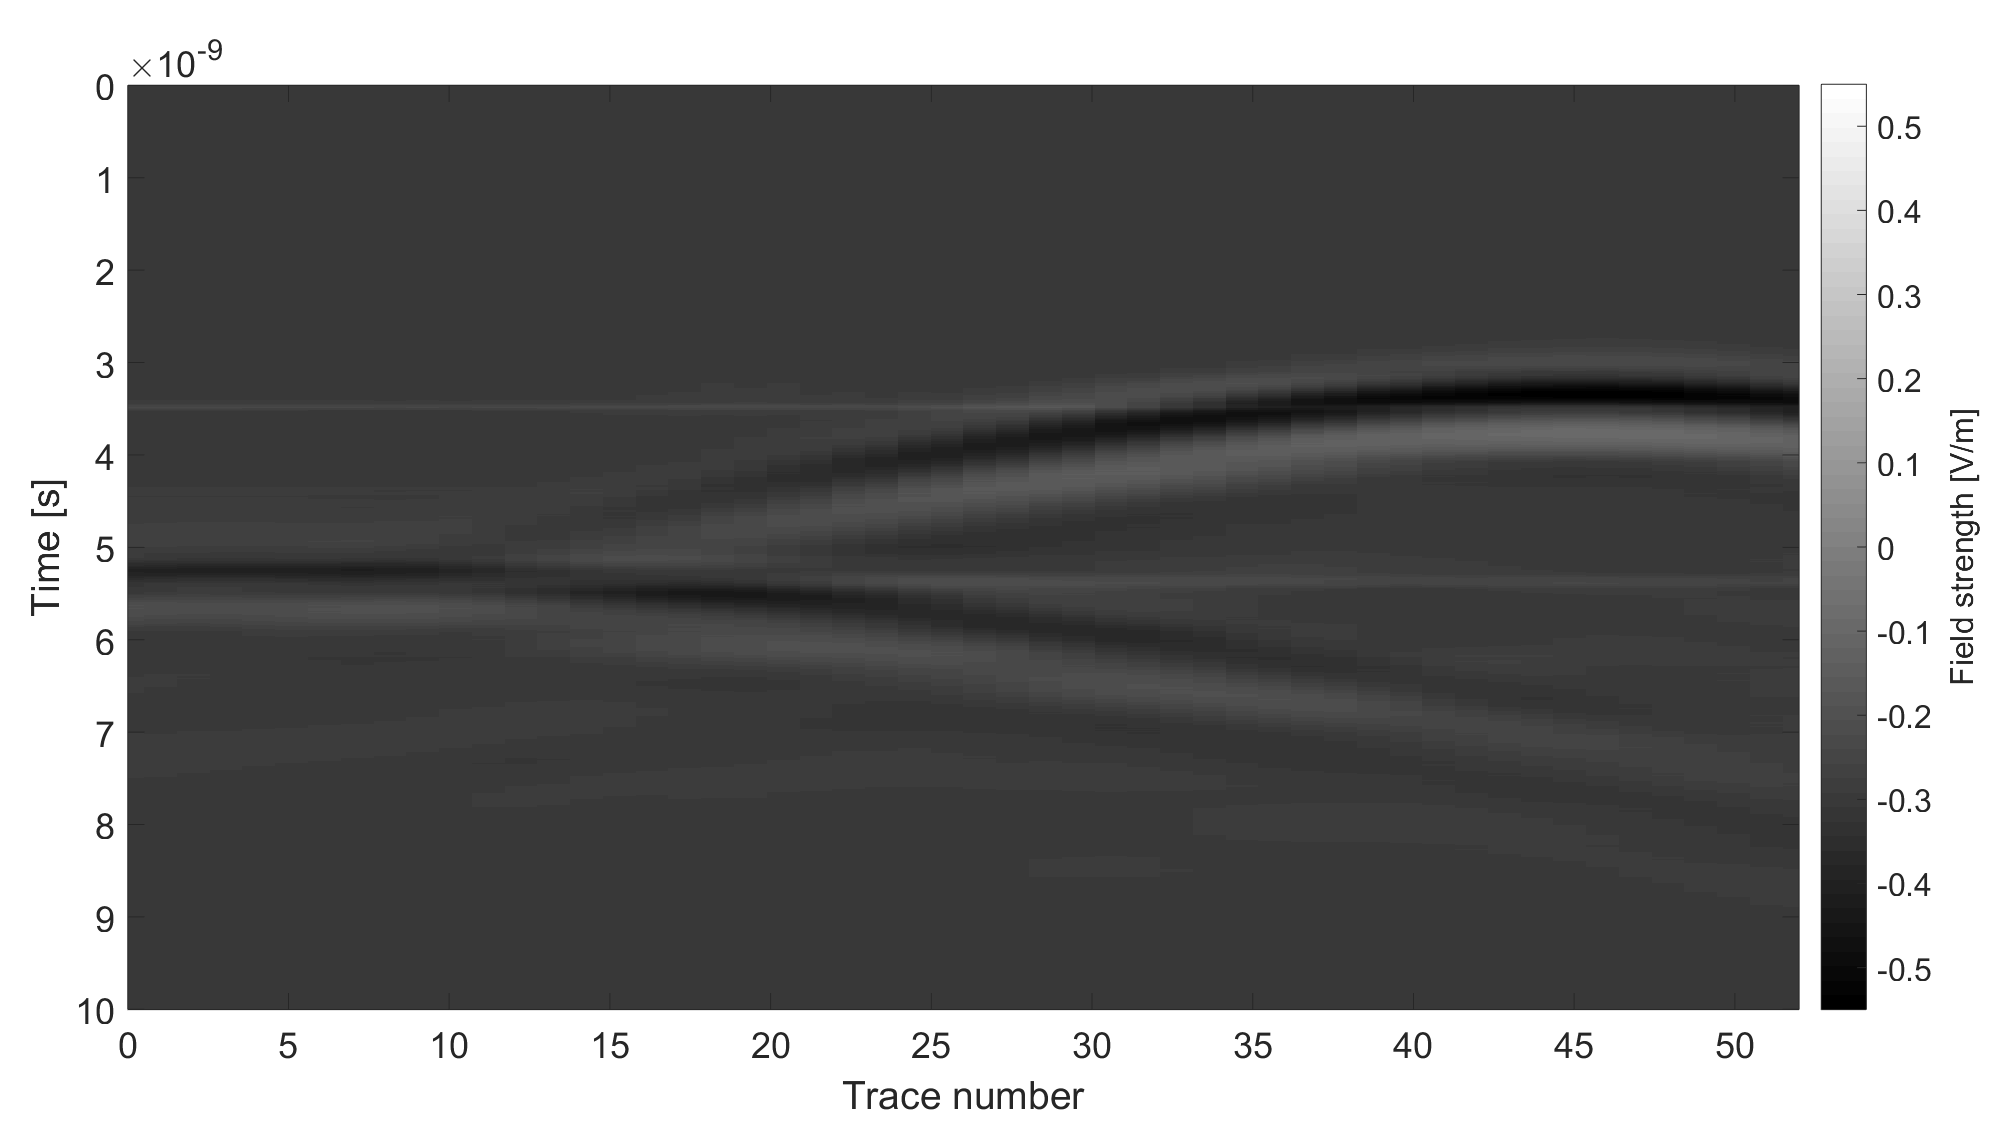
\includegraphics[width=0.47\textwidth, keepaspectratio,valign=c]{chapter2/images/mala_2_barras_bscan_sparse.png}
}

\caption{Señal Barras Metálicas Ez}
\label{fig:barraMetalIdeal}


\end{figure}

En la \figurename{ \ref{fig:barraMetalIdeal}} se puede observar la comparación de las señal ideal que debe generar únicamente las barras metálicas  con la señal resultante al aplicar RPCA.  Respecto a la \tablename{ \ref{tab:corrcoef1}} indica que la traza B (sparse) tiene una similitud del 84.8\% con respecto a la traza ideal.


\subsubsection{Mean Substraction}

Es uno  de los métodos de pre-procesamiento más simples para eliminar las componentes de baja frecuencia que se encuentran presentes en un conjunto de datos. \cite{round_Clutter_Removal_in_GPR_Surveys}. Se puede notar ${ e }_{ 1 }{ \left( t \right)  },{ e }_{ 2 }{ \left( t \right)  },{ e }_{ 3 }{ \left( t \right)  },...,{ e }_{ n }{ \left( t \right)  }$ como el conjunto de trazas A sobre M observaciones en un instante de tiempo t.  Cada traza contiene diferentes valores proveniente del acople entre antenas, la interferencia de las multiples señales de la interfaz aire-suelo y las señales reflejadas por los objetos enterrados (targets). La señal recolectada en una n-ésima posición puede ser notada como:

\begin{equation}
{ e }_{ n }{ \left( t \right)  }={ e }_{ na }{ \left( t \right)  }+{ e }_{ nw }{ \left( t \right)  }+{ e }_{ nt }{ \left( t \right)  }
\end{equation}

Donde ${ e }_{ na }{ \left( t \right)  }$ corresponde al acople entre antenas, ${ e }_{ nw }{ \left( t \right)  }$ la señal de las reflexiones del suelo y ${ e }_{ nt }{ \left( t \right)  }$ las reflexiones de los objetos.

Para aplicar este algoritmo se busca reducir o eliminar las componentes ${ e }_{ na }{ \left( t \right)  }$ y ${ e }_{ nw }{ \left( t \right)  }$ ya que son fuentes de ruido. Al eliminar las fuentes de ruido se puede tener una imagen ``mejorada'' de las señales originadas por los objetos enterrados.
La ecuación de este algoritmo de pre procesamiento  es:
\begin{equation}
{ e }_{ AVn }{ \left( t \right)  }={ e }_{ n }{ \left( t \right)  }-\quad \frac { 1 }{ M }  \sum _{ m=1 }^{ M }{ { e }_{ n }{ \left( t \right)  } } 
\end{equation}

Donde ${ e }_{ AVn }$ corresponde a valor de la traza extraída,  ${ e }_{ n }$ a los datos de la traza A en la n-ésima iteración y M el número de observaciones (Cuantas trazas A esta compuesta la traza B).
\newpage
\subsubsubsection{\textbf{Implementación Mean Substraction en trazas gprMax}}

Se desarrolló un programa en Matlab  para seleccionar un conjunto de trazas B y aplicarle a cada una de ellas el algoritmo Mean Substraction, el programa crea una carpeta nueva con los valores del resultado del algoritmo.

\begin{lstlisting}[ basicstyle=\tiny] 
% get_all_Bscans_MeanSubstraction.m
% Los Andes University
% Creaded By: Luis Eduardo Quibano Alarcon
% E-mail: le.quibano@uniandes.edu.co
% Description: This Script  opens a specific amoun of  Bscans in order to
%              apply them the MEAN SUBSTRACTION algotrithm in all field components of
%              each A-scaN.
% MeanSubstraction Algorithm: https://doi.org/10.1109/JSTARS.2013.2287016
%                             https://pdfs.semanticscholar.org/783c/70ff019d8f225ad9bc2aa61ba614f09628ba.pdf

clear all
close all
clc

[filename, pathname] = uigetfile('*.out', 'Select gprMax B-scans output files','MultiSelect','on');
fullfilename = strcat(pathname, filename);

filename = cellstr(filename);
pathname = cellstr(pathname);
fullfilename = cellstr(fullfilename);

%Extraigo todos los campos de los A-scan seleccionados y luego los guardo
%en la matriz del objeto fields{i}

fullfilenameMeanS = fullfilename;
filenameMeanS=filename;
%%CREATE A COPY OF B-SCAN WITH NAME LOW RANK
%%CREATE A COPY OF A-SCAN WITH NAME LOW RANK
if exist(strcat(pathname{1},'/MeanSubstraction')) == 7
    rmdir(strcat(pathname{1},'/MeanSubstraction'), 's')
end
mkdir(strcat(pathname{1},'/MeanSubstraction'))
pathToSave=strcat(pathname{1},'/MeanSubstraction')


for i=1:length(fullfilenameMeanS)
    if filename{i} ~= 0
        nameSplit = split(filenameMeanS{i},'.');
        nameSplit= nameSplit(1);
        nameSplit= strcat(pathToSave,'/',nameSplit{1});
        nameSplit=strcat(nameSplit(1:end),'_MeanS','.out');
        fullfilenameMeanS{i}=nameSplit ;
        copyfile(fullfilename{i}, nameSplit);
    end
end


if length(fullfilenameMeanS) ~=0
    for i=1:length(fullfilenameMeanS)
        if filename{i} ~= 0
            iterations = double(h5readatt(fullfilenameMeanS{i}, '/', 'Iterations'));
            dt = h5readatt(fullfilenameMeanS{i}, '/', 'dt');
            
            ExFieldPath = strcat('/rxs/rx1/', 'Ex');
            EyFieldPath = strcat('/rxs/rx1/', 'Ey');
            EzFieldPath = strcat('/rxs/rx1/', 'Ez');
            HxFieldPath = strcat('/rxs/rx1/', 'Hx');
            HyFieldPath = strcat('/rxs/rx1/', 'Hy');
            HzFieldPath = strcat('/rxs/rx1/', 'Hz');
            
            
            ExAllScans = h5read(fullfilenameMeanS{i}, ExFieldPath);
            tam = size(ExAllScans);
            longi= tam(1);
            EyAllScans = h5read(fullfilenameMeanS{i}, EyFieldPath);
            EzAllScans = h5read(fullfilenameMeanS{i}, EzFieldPath);
            HxAllScans = h5read(fullfilenameMeanS{i}, HxFieldPath);
            HyAllScans = h5read(fullfilenameMeanS{i}, HyFieldPath);
            HzAllScans = h5read(fullfilenameMeanS{i}, HzFieldPath);
            
            %Aplly Mean Substractions
            ExAllScansMeanS=  ExAllScans - sum((ExAllScans))/longi;
            EyAllScansMeanS=  EyAllScans - sum((EyAllScans))/longi;
            EzAllScansMeanS=  EzAllScans - sum((EzAllScans))/longi;
            HxAllScansMeanS=  HxAllScans - sum((HxAllScans))/longi;
            HyAllScansMeanS=  HyAllScans - sum((HyAllScans))/longi;
            HzAllScansMeanS=  HzAllScans - sum((HzAllScans))/longi;
 
            %Write in H5file
            h5write(fullfilenameMeanS{i}, ExFieldPath,ExAllScansMeanS);
            h5write(fullfilenameMeanS{i}, EyFieldPath,EyAllScansMeanS);
            h5write(fullfilenameMeanS{i}, EzFieldPath,EzAllScansMeanS);
            h5write(fullfilenameMeanS{i}, HxFieldPath,HxAllScansMeanS);
            h5write(fullfilenameMeanS{i}, HyFieldPath,HyAllScansMeanS);
            h5write(fullfilenameMeanS{i}, HzFieldPath,HzAllScansMeanS);
            
            
        end
    end
    
end

\end{lstlisting}


\begin{figure}[H]  
\centering
\subfigure[ Modelo Original ]{
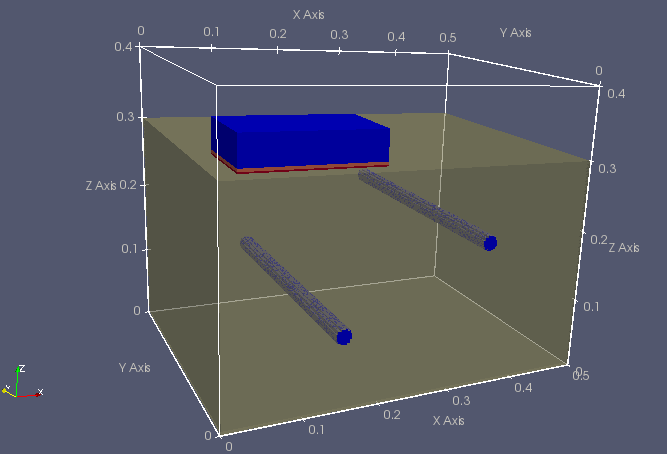
\includegraphics[width=0.25\textwidth, keepaspectratio,valign=c]{chapter2/images/mala_2_barras.png}
\label{fig:subfig_mala2_barras_mod}
}\\
\subfigure[ Bscan datos originales ]{
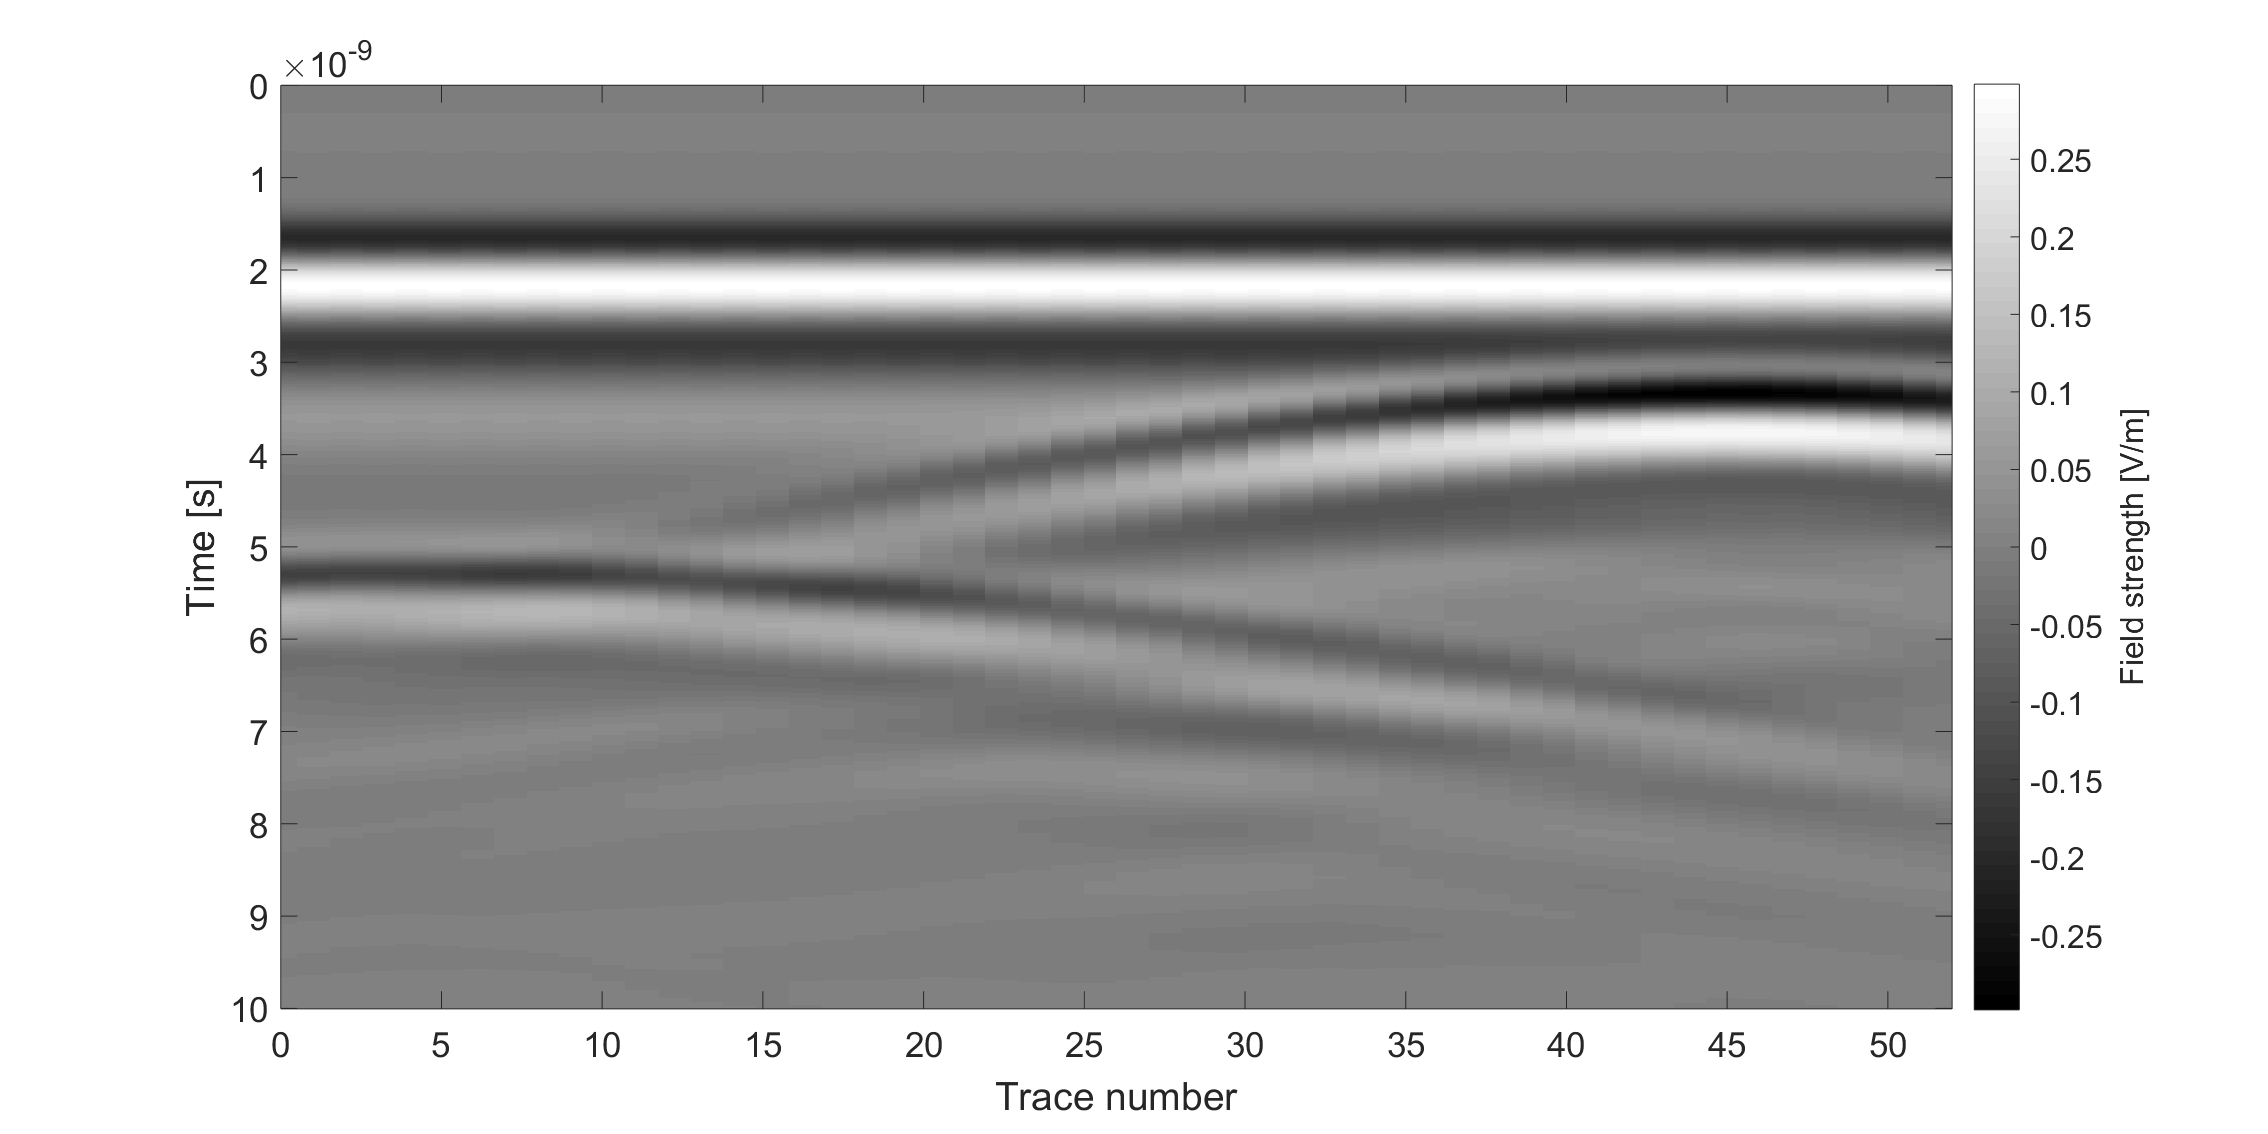
\includegraphics[width=0.45\textwidth, keepaspectratio,valign=c]{chapter2/images/mala_2_barras_bscan.png}
\label{fig:subfig1xampleCscan1GSSI}
}
\subfigure[ Bscan Mean Substraction ]{
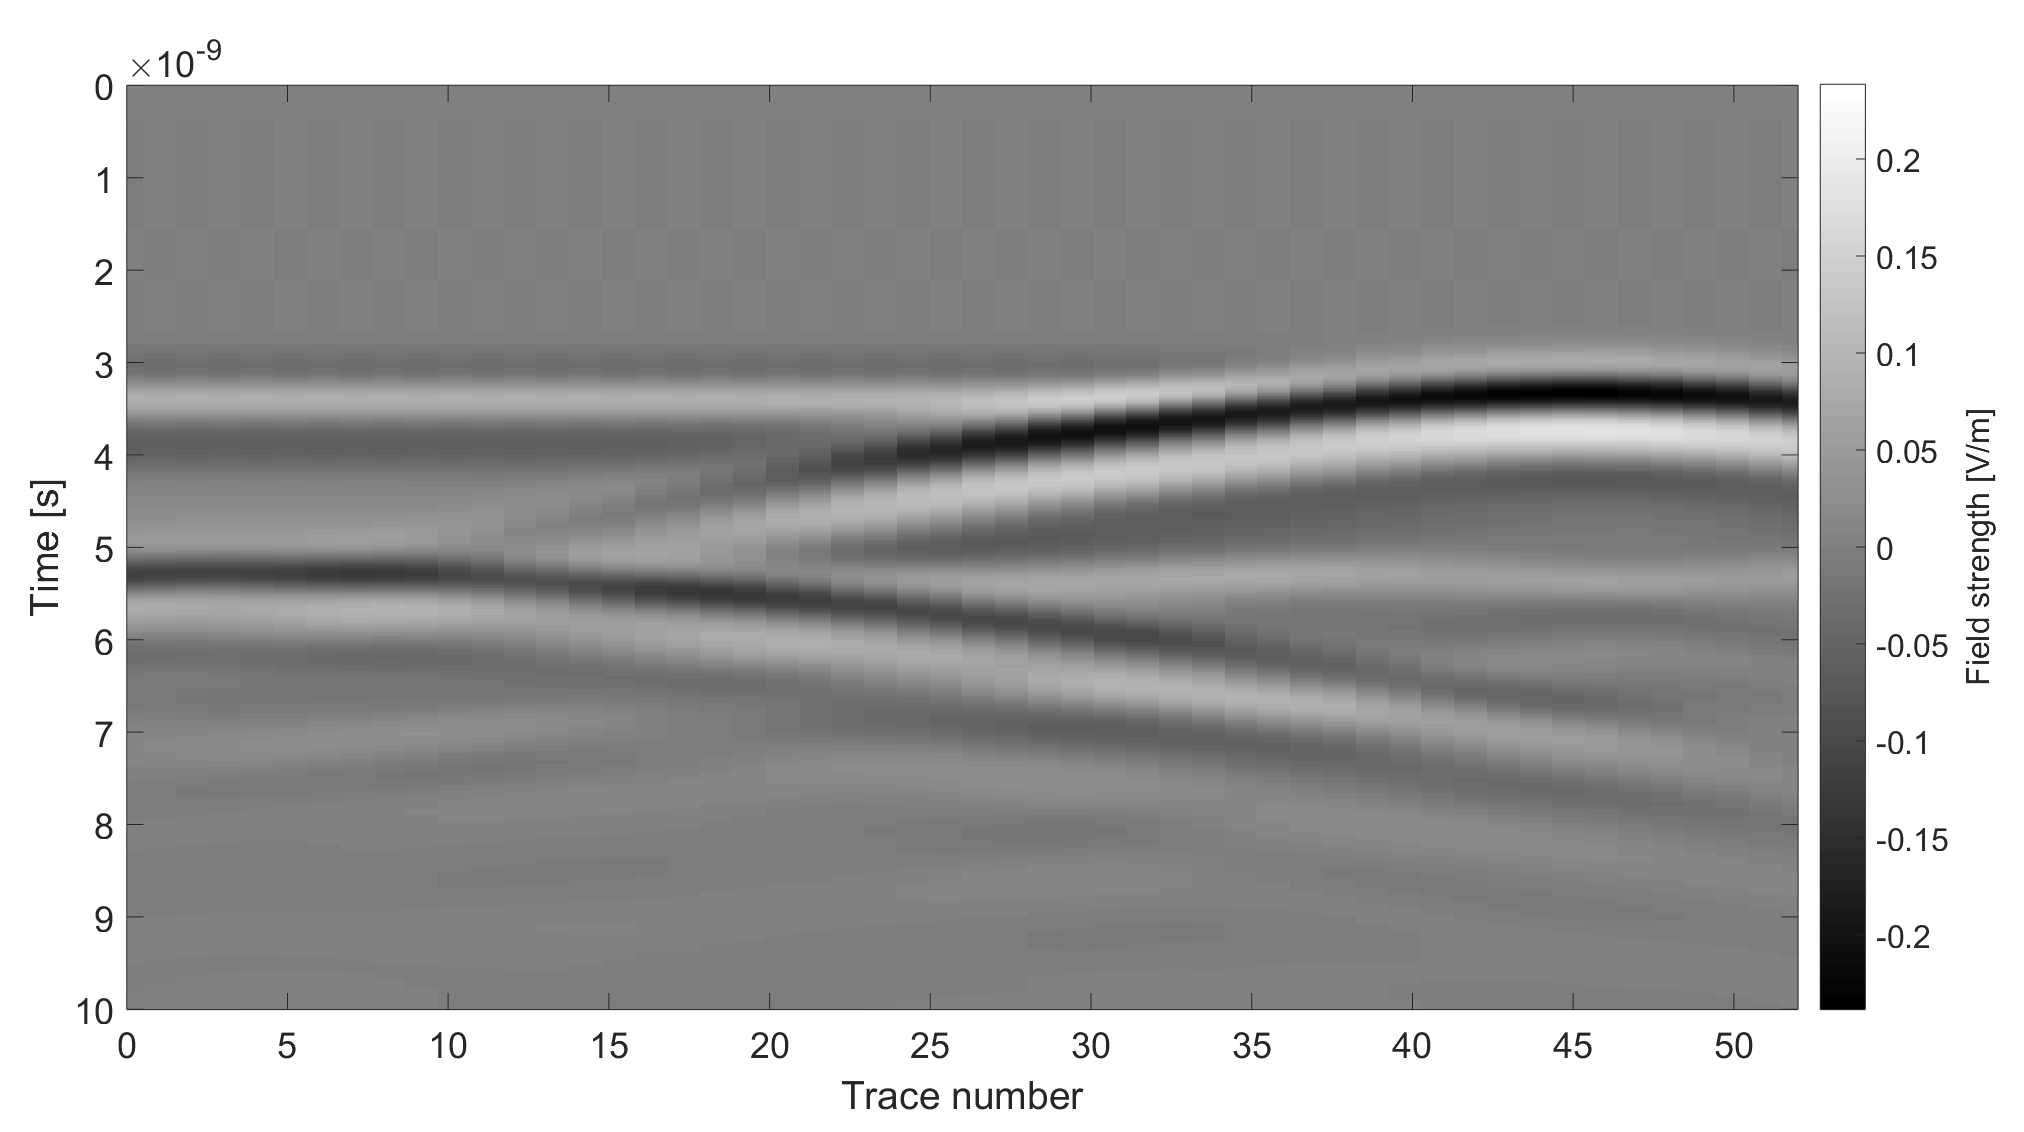
\includegraphics[width=0.45\textwidth, keepaspectratio,valign=c]{chapter2/images/mala_2_barras_bscan_meanSubstraction.png}
\label{fig:subfig2exampleCscan1GSSI}
}
\caption{Mean Substraction sobre trazas B en campo Ez}
\label{fig:bscanMeanSubs1}
\end{figure}


\begin{table}[H]
\begin{center}
\caption{Similitud entre resultados aplicando Mean Subtraction} \label{tab:corrcoefMean}
\begin{tabular}{l|c}
 & \multicolumn{1}{l}{\textbf{Índice de Correlación}} \\ \hline
\textbf{(Ex ideal,Ex MeanS)} & NaN \\
\textbf{(Ey ideal,Ey MeanS)} & 0.8015 \\
\textbf{(Ez ideal,Ez MeanS)} & 0.8016 \\
\textbf{(Hx ideal,Hx MeanS)} & 0.7684 \\
\textbf{(Hy ideal,Hy MeanS)} & 0.8580 \\
\textbf{(Hz ideal,Hz MeanS)} & 0.8639
\end{tabular}
\end{center}
\end{table} 


\begin{figure}[H]  
\centering
\subfigure[ Bscan Ideal ]{
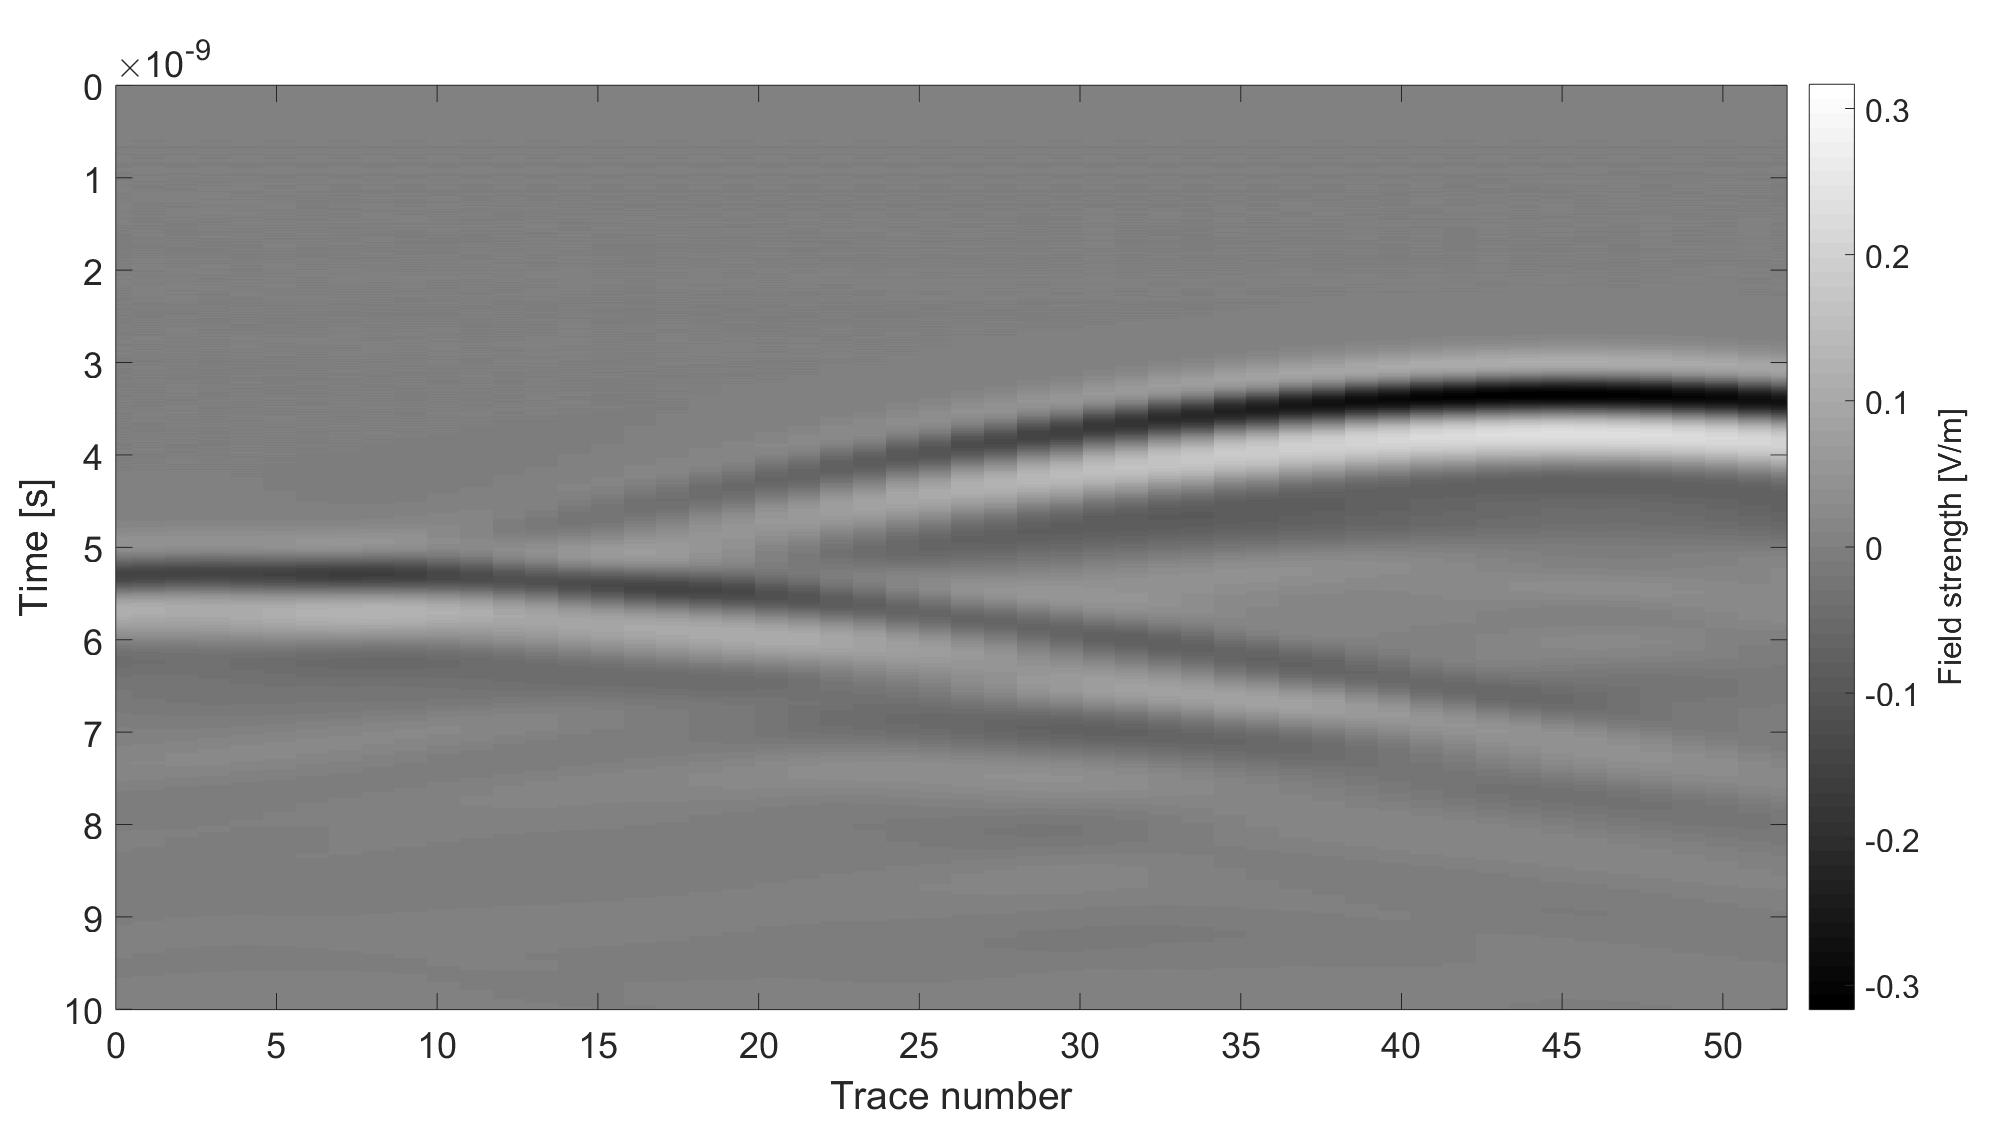
\includegraphics[width=0.47\textwidth, keepaspectratio,valign=c]{chapter2/images/mala_2_barras_bscan_sparse_ideal.png}
\label{fig:subfig2exampleCscan1GSSI}
}
\subfigure[Bscan Mean Substraction ]{
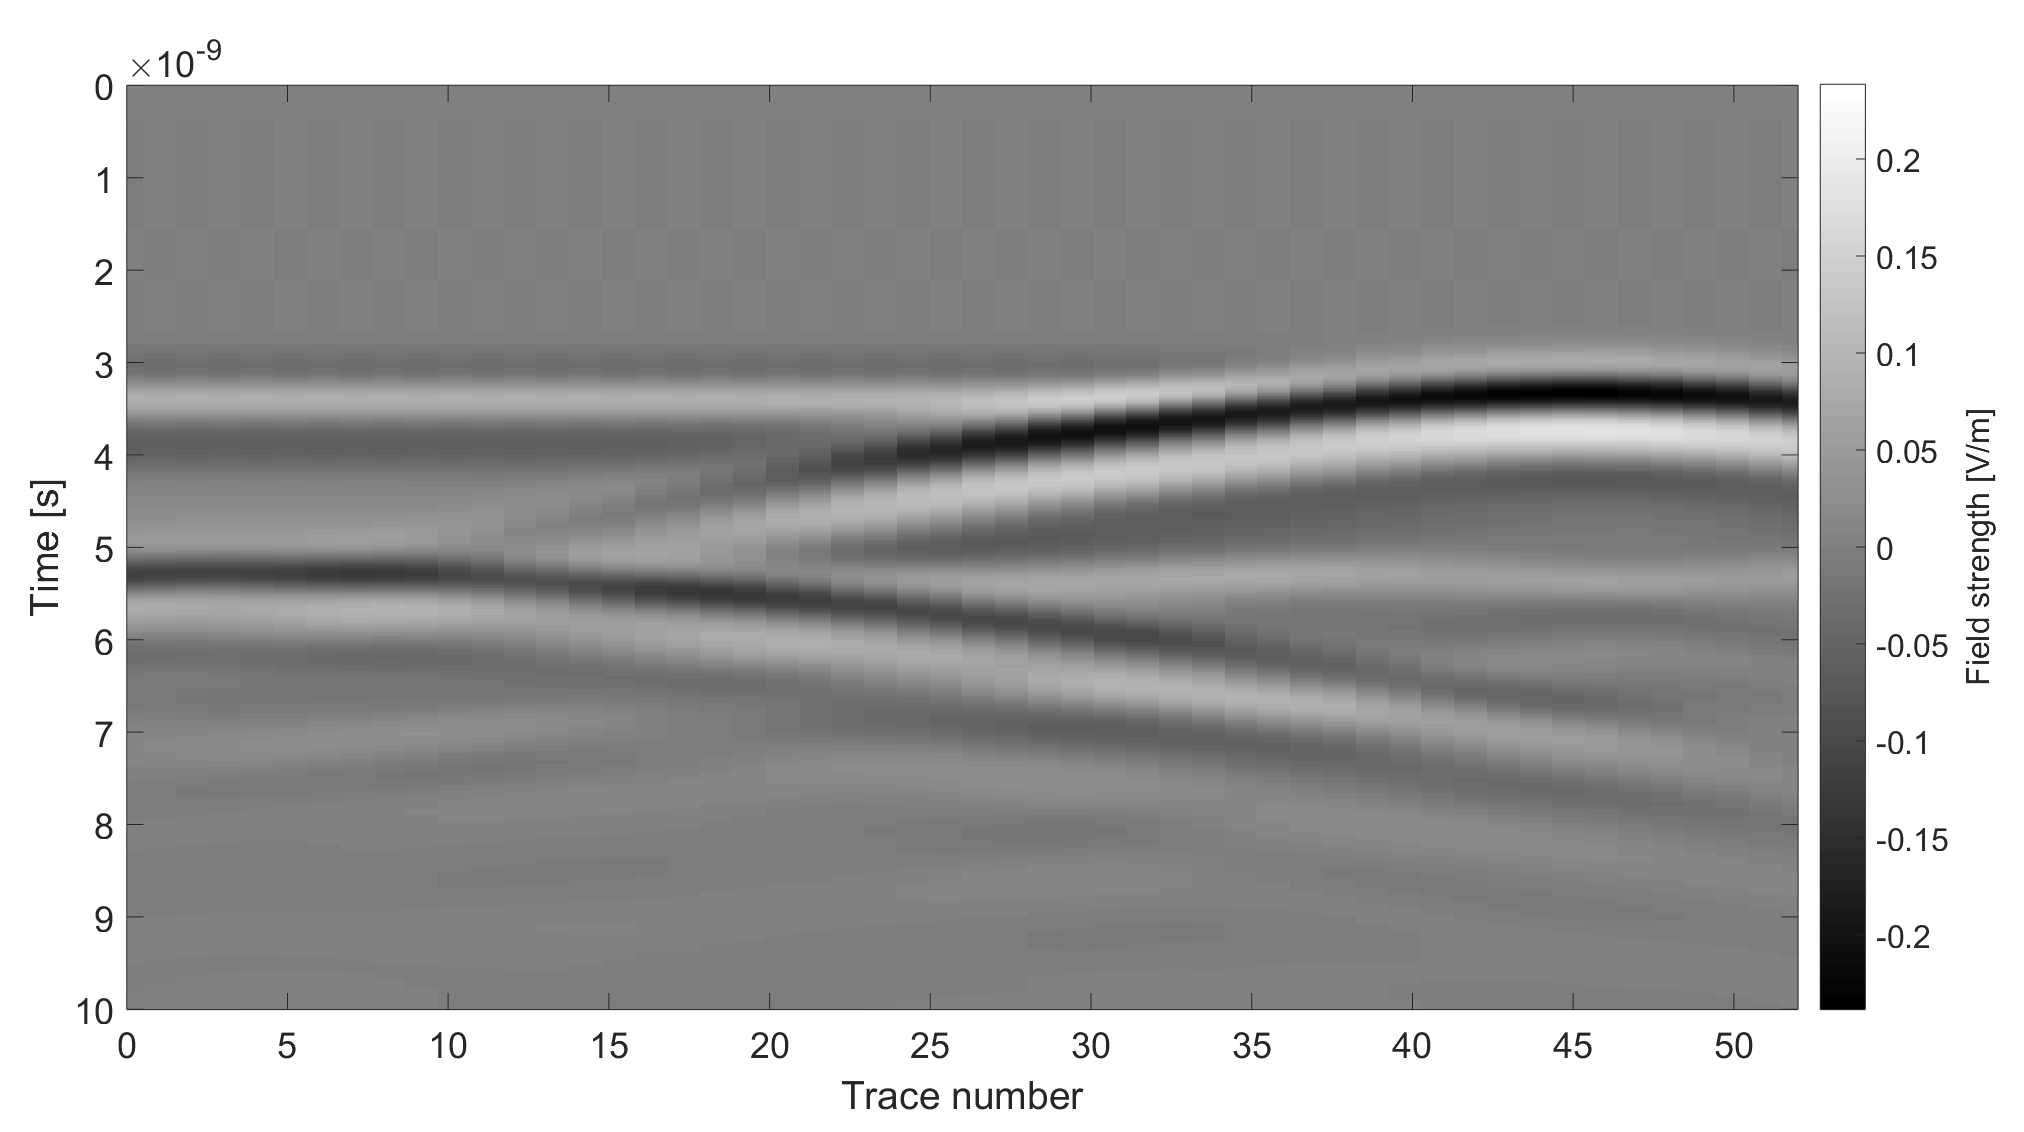
\includegraphics[width=0.47\textwidth, keepaspectratio,valign=c]{chapter2/images/mala_2_barras_bscan_meanSubstraction.png}
}
\caption{Señal Barras Metálicas Ez}
\label{fig:barraMetalIdeal}
\end{figure}

 
\subsubsection{Contrast Stretching}

\subsubsection{Entropy Based-Time Gating}
\subsubsection{Subspace Projection}




